\documentclass[10pt,twocolumn,letterpaper]{article}

\usepackage{cvpr}
\usepackage{times}
\usepackage{epsfig}
\usepackage{graphicx}
\usepackage{amsmath}
\usepackage{amssymb}

\usepackage{media9}
\usepackage{filecontents}
%\usepackage{geometry}
\usepackage{caption}
\usepackage{subcaption}

% Include other packages here, before hyperref.

% If you comment hyperref and then uncomment it, you should delete
% egpaper.aux before re-running latex.  (Or just hit 'q' on the first latex
% run, let it finish, and you should be clear).
\usepackage[breaklinks=true,bookmarks=false]{hyperref}

\cvprfinalcopy % *** Uncomment this line for the final submission
\def\httilde{\mbox{\tt\raisebox{-.5ex}{\symbol{126}}}}

% Pages are numbered in submission mode, and unnumbered in camera-ready
%\ifcvprfinal\pagestyle{empty}\fi
\setcounter{page}{1}
\begin{document}

%%%%%%%%% TITLE
\title{Volumetric Capture}

\author{Marcel Bruckner\\
{\tt\small marcel.bruckner@tum.de}
\and
Kevin Bein\\
{\tt\small kevin.bein@tum.de}\\[0.5em]
Technische Universit\"at M\"unchen
\and
Moiz Sajid\\
{\tt\small moiz.sajid@tum.de}
}

\maketitle
%\thispagestyle{empty}

\newcommand{\intel}{Intel\textsuperscript{\textcopyright}}
\newcommand{\fref}[1]{\mbox{Figure~\ref{#1}}}
\newcommand{\tref}[1]{\mbox{Table~\ref{#1}}}
\newcommand{\sref}[1]{\mbox{Section~\ref{#1}}}
\newcommand{\rscamera}{\intel{} RealSense\texttrademark{} Depth Camera~D415 \cite{DepthCameraD415}}
\newcommand{\aruco}{ArUco~markers~\cite{ArUco}}
\newcommand{\charuco}{ChArUco~markers~\cite{ChArUco}}
\newcommand{\opencv}{OpenCV~\cite{OpenCV}}
\newcommand{\opengl}{OpenGL~\cite{OpenGL}}

%%%%%%%%% ABSTRACT
\begin{abstract}
   Our goal in this project is to get a real time mesh reconstruction of dynamic scenes using a multi view camera capture setup. We use three Intel RealSense D415 depth cameras for RGB-D data capturing which are calibrated using known correspondences from markers. The data is fused into a voxelgrid representing the implicit surface and following a marching cubes algorithm is performed for the final surface extraction. Both qualitative and quantitative results are presented.   
\end{abstract}


\begin{figure}[t]
	\begin{center}
		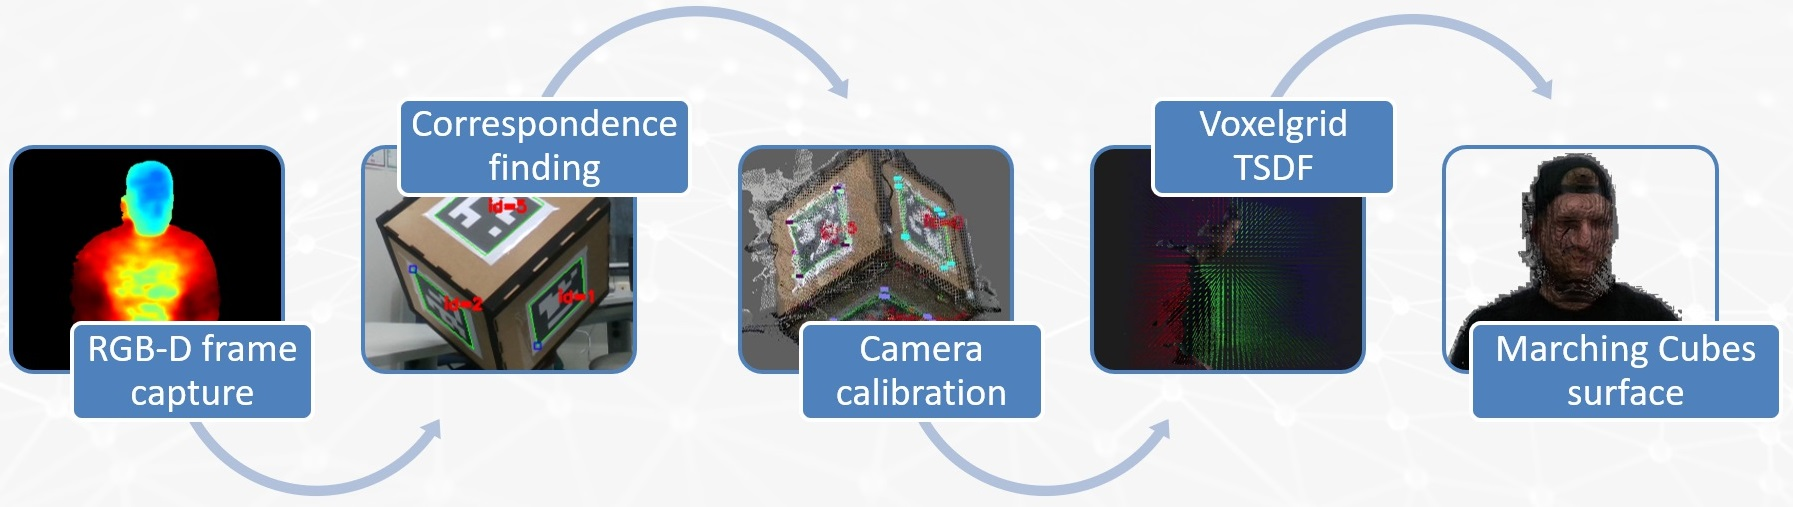
\includegraphics[width=1.0\linewidth]{imgs/pipeline}
	\end{center}
	\caption{Reconstruction pipeline used in this project: RGB-D Frame Capture, Correspondence Finding, Camera Calibration, Voxelgrid TSDF, Marching Cubes}
	\label{fig:reconstruction-pipeline}
\end{figure}

%%%%%%%%% BODY TEXT
\section{Introduction}

Volumetric Capture is an extensively researched topic where the goal is to get an accurate 3D reconstruction of dynamic scenes in real time. The first work in the area was done by Cureless and Levoy~\cite{Authors4} in which they integrated data from one range image into a cumulative weighted signed distance function. KinectFusion~\cite{Authors5} was another milestone in this area which proposed a real time mapping system of indoor scenes using a single depth camera. DynamicFusion~\cite{Authors6} handles non-rigid scenes and reconstruction over time. Our work mostly focuses on reconstructing dynamic scenes on a per frame basis.\\
One application area of our project is Holoportation~\cite{Authors7} where 3D reconstructed models are used for VR interactions between two persons over huge distances.

\begin{figure}
	\centering
	\begin{subfigure}[t]{.315\linewidth}
		\centering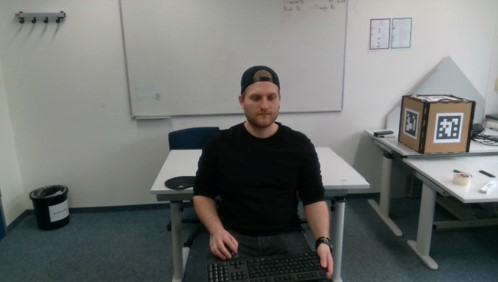
\includegraphics[width=0.9\linewidth]{imgs/rgb}
		\caption{RGB Image}
		\label{fig:rgb}
	\end{subfigure}
	\begin{subfigure}[t]{.315\linewidth}
		\centering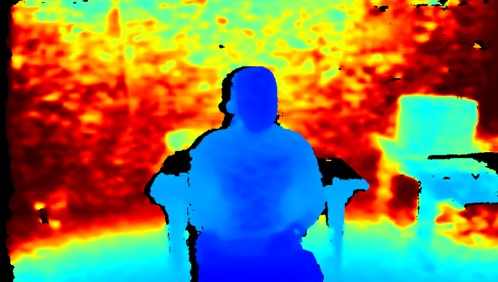
\includegraphics[width=0.9\linewidth]{imgs/depth}
		\caption{Depth Image}
		\label{fig:depth}
	\end{subfigure}
	\begin{subfigure}[t]{.315\linewidth}
		\centering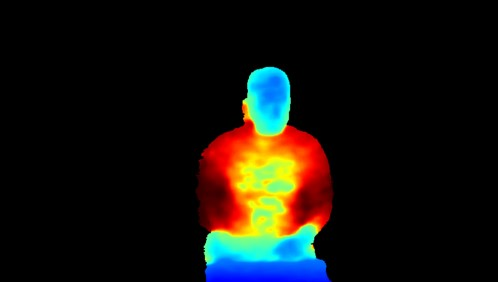
\includegraphics[width=0.9\linewidth]{imgs/threshold}
		\caption{Threshold filter}
		\label{fig:threshold}
	\end{subfigure}  
	\caption{The color and depth images captured by the \mbox{cameras}}
	\label{fig:rgbd-data}
\end{figure}
%------------------------------------------------------------------------
\section{Reconstruction Pipeline}
\label{sec:reconstruction-pipeline}
To perform the real time 3D reconstruction we implemented the pipeline which is exemplary displayed in \fref{fig:reconstruction-pipeline} and described in the following section.\\
All tests were performed on a Laptop with an Intel\textsuperscript{\textregistered} Core\texttrademark{} \mbox{i7-6700HQ} CPU @ 2.60GHz~\cite{CPU}, 40GB of DDR4 RAM and a Nvidia GeForce GTX 970M~\cite{GTX970}.

%-------------------------------------------------------------------------
\subsection{RGB-D Frame Capture}
We use three \rscamera{} for our capture setup which work on the concept of active stereo depth. Two cameras are placed on the sides of the camera and the depth is calculated from a triangulation using the displacement. An infrared pattern is projected into the scenweree to enhance the details.\\
We process the depth images using a threshold filter which discards pixels that are above or below a threshold set during runtime. We also tried different hole-filling, spatial and edge enhancing filters that did not improve the results and are not used in the final reconstruction.\\
\fref{fig:rgbd-data} displays the raw RGB-D images and the filtered depth image.

We tried to extend the three camera setup with a fourth one but were not able to integrate it due to bandwidth limitations. Furthermore, we had to limit the color and depth resolutions as well as framerates to enable three cameras and to allow a processing of the data in real time. The resolution we used for the color and depth stream is 848x480 px at 30 frames per second. \cite{RealSenseWhitepaper} gives more detail about the limitations of the cameras in a multi camera setup.
\newpage
The RGB-D images from the three cameras are time synchronized~\cite{RealSenseWhitepaper} what improves the results of the following camera calibration and the final mesh reconstruction.

\intel{} provides an excellent SDK~\cite{RealSenseSDK}, good support and updates for its API which made it easy to use the cameras.

%------------------------------------------------------------------were-------
\subsection{Correspondence Finding}
We use \aruco{} to find correspondences between the three camera streams. These markers have a unique identifier and can easily be detected in every color image using the \opencv{} library.\\
The markers are mounted on a wooden cube box as shown in \fref{fig:cube}.

By placing the cameras such that each one is looking on one of the cubes corners we can assure that in every color image three markers are visible. This also ensures that between every pair of cameras we have an overlap of two markers for which the eight corner positions are detected sub pixel perfect. This gives us a total of $8*3=24$ constraints between every pair of cameras which are used in the next step to estimate the relative transformation between the markers.

It is also important to mention here that we tried \charuco{} which are a mixture of \aruco{} and a chessboard pattern which allow simultaneous detection and pose estimation. However, the \charuco{} did not give us good pose results and slowed down the calculation (\tref{tab:camera-calibration}), so we stick to \aruco{}. 
%
%
\begin{figure}[t]
	\begin{center}
		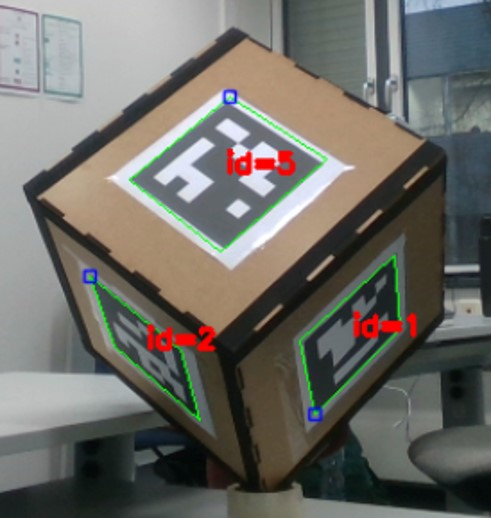
\includegraphics[width=0.6\linewidth]{imgs/cube}
	\end{center}
	\caption{Marker cube with the detected markers highlighted in green and their unique identifiers (red).}
	\label{fig:cube}
\end{figure}
%
%
%-------------------------------------------------------------------------
\subsection{Camera Calibration}
We use the known marker positions in the color image and combine them with the depth information to calculate the 3D position of the marker corners. As we ensure to have an overlap of two markers between every pair of cameras we now have $8*3=24$ constraints (8 markers each with a x, y and z value). The 3D positions are then fed into two alignment algorithms to find the relative transformations between the cameras and to align the pointclouds based on the results.
%
%-------------------------------------------------------------------------
\subsubsection{Procrustes}
The Procrustes algorithm aligns two pointclouds using known correspondences by estimating the relative translation and rotation between the two sets of points.
\paragraph{Translation}
We calculate the center of gravity for every pointcloud by summing up the individual point positions and dividing by the number of points. This gives us for every set of points the mean point. The translation is then estimated by the difference between the centers of gravity.
\begin{equation}
	T_{ij} = C_i - C_j
\end{equation}were
\paragraph{Rotation}
The rotation between two pointclouds can be estimated by optimizing over the unknown rotation $R_{ij}$. This is done by minimizing the mean squared error between the set of points $X_i$ and the $X_j$.
\begin{equation}
	\min_{R_{ij}} || X_i - R_{ij} X_j ||^2_2
\end{equation}
Fortunately there exists a closed form solution for the rotation $R_{ij}$ which is based on the singular value decomposition of the matrix $X_i^T X_j$.
\begin{align}
	X_i^T X_j &= U \Sigma V^T \\
	R_{ij} &= UV^T
\end{align}
\tref{tab:camera-calibration} displays the duration and mean squared error values after the Procrustes alignment. It shows a still fairly high error, so we had to further align the pointclouds.
%
\subsubsection{Point-to-Point Error}
In order to further improve the alignment that we get from Procrustes we use a Point-to-Point correspondence error. We optimize for the relative translation $T_{ij}$ and rotation $R_{ij}$ over every pair of camera frames $i$ and $j$ and in each of these for the known correspondences $k$. We came up with the following energy term:
\begin{equation}\label{eq5}
\min_{T_{ij}, R_{ij}} \sum_{i}^{frame}\sum_{j}^{frame}\sum_{k}^{corres.} || X_{ik} - T_{ij}R_{ij}*X_{jk} ||_2^2
\end{equation}
A comparison of the results from this optimization is given in \tref{tab:camera-calibration}. It shows that the mean squared error is much lower using the transformation from the Point-to-Point optimization. On the other side it displays an increase of the duration for the estimation as it is an iterative optimization algorithm, but as the pose estimation is done only once in the beginning the increase is negligible.
%
%-------------------------------------------------------------------------
\subsection{Voxelgrid TSDF}
We calculate a truncated signed distance field (TSDF) based on a voxelgrid to represent the implicit surface of the aligned pointclouds. The voxelgrid is a three-dimensional cuboid structure with points (voxels) filling it on a grid at a given resolution. An exemplary voxelgrid is displayed in \fref{fig:voxelgrid}. 

We fuse the aligned pointclouds into the voxelgrid by iterating over every voxel and projecting it into the depth frame of the camera. We can now lookup the surface depth value $z_{depth}$ at the projected position in the depth image and compare it to the depth of the voxel. This gives us the distance $d_i$ of the voxel to the surface in the $i$-th camera frame:
\begin{equation}\label{eq1}
d_i = z_{voxel} - z_{depth,i}
\end{equation}
The final TSDF value is then calculated by truncating the distance with a given threshold $t$:
\begin{equation}
	tsdf_i = min(max(-t, d_i), t)
\end{equation}
We do this integration for all three sets of points coming from the cameras. To get a valid representation of the implicit surface for all pointclouds we perform a weighted averaging: 
\begin{equation}\label{eq2}
tsdf_{i+1}=\frac{tsdf_{i} * weight}{weight+1}
\end{equation}

As we compute the TSDF values for a large number of voxels we had to parallelize the calculations using the GPU~(\sref{sec:reconstruction-pipeline}). Since we are using \opengl{} for the rendering we decided to use \opengl{} compute shaders~\cite{Authors1} for hardware accelerated parallelization. \tref{tab:voxelgrid} displays the duration for integrating all three camera frames into the voxelgrid at different resolutions and their respective number of voxels. \\

\begin{figure}[t]
\begin{center}
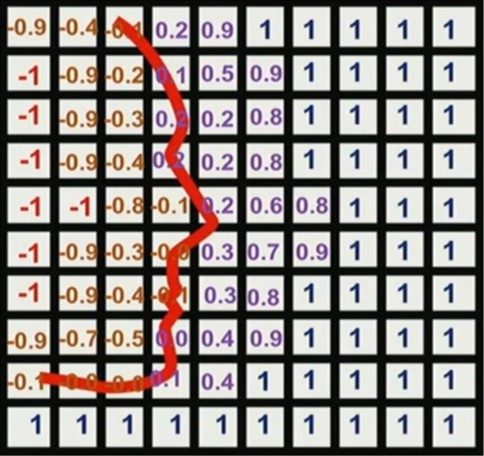
\includegraphics[width=0.6\linewidth]{imgs/tsdf}
\end{center}
 \caption{A two-dimensional voxelgrid with an implicit surface (red) and the respective TSDF values. The TSDF values are positive outside of the surface and negative inside. The zero-crossing represents the surface.}
 \label{fig:voxelgrid}
\end{figure}

%-------------------------------------------------------------------------
\subsection{Surface Extraction}
For the iso-surface extraction, we used the Marching Cubes algorithm which converts the implicit surface representation to a polygonal mesh. We then iterated over the voxelgrid cells to determine the zero crossings and looked up the triangulation in the Marching Cubes table. This gives us the trianguled mesh as an final output. With a lower voxel resolution and more grid points, we were able to get more finer reconsturction. Again we had to utilize the OpenGL Compute Shader in order to achieve real time results because the computations on the CPU were really slow.

Intially, we had voxelgrid points that were not initialized because they were outside the camera view. As a result, we had a huge number of artefacts in the final mesh reconstruction which took a lot of time to figure out. We implemented a two pass OpenGL Compute Shader. In the first pass, we counted the number of triangles that will generated and only allocated space for them. In the second pass, we generate the triangles. We do this because the upper bound for the number of generated triangle is five times the number of voxelgrid points. For example if we have 200x200x200 grid points with a 5 millimeter voxel resolution, we roughly had 40 million number of possible triangles. We only generated a fraction of these triangles after the the triangle counting OpenGL Compute Shader pass. For a voxel resolution of 5mm resolution, the Marching Cubes algorithm took 15 milliseconds which was real time capable. For 3 millimeter resolution, the results were not real time capable however, we were to get fine mesh reconstructions.  The Table~\ref{tab:table2} summarizes the time comparisons between different voxel resolution. The Table~\ref{tab:table3} summarizes the time comparisons for running Marching Cubes between different voxel resolutions. 

%------------------------------------------------------------------------
\section{Results}
The results that we get using one camea are really good as can be seen in Figure \ref{fig:res1}. Figure \ref{fig:res2} displays the triangulation results using one camera. However, we get artefacts when we use all three camera streams. The which artefacts which are mostly visible around the edges can be seen in Figure \ref{fig:res3}. This suggests that the camera pose parameters can be improved further.

\begin{figure}[t]
\begin{center}
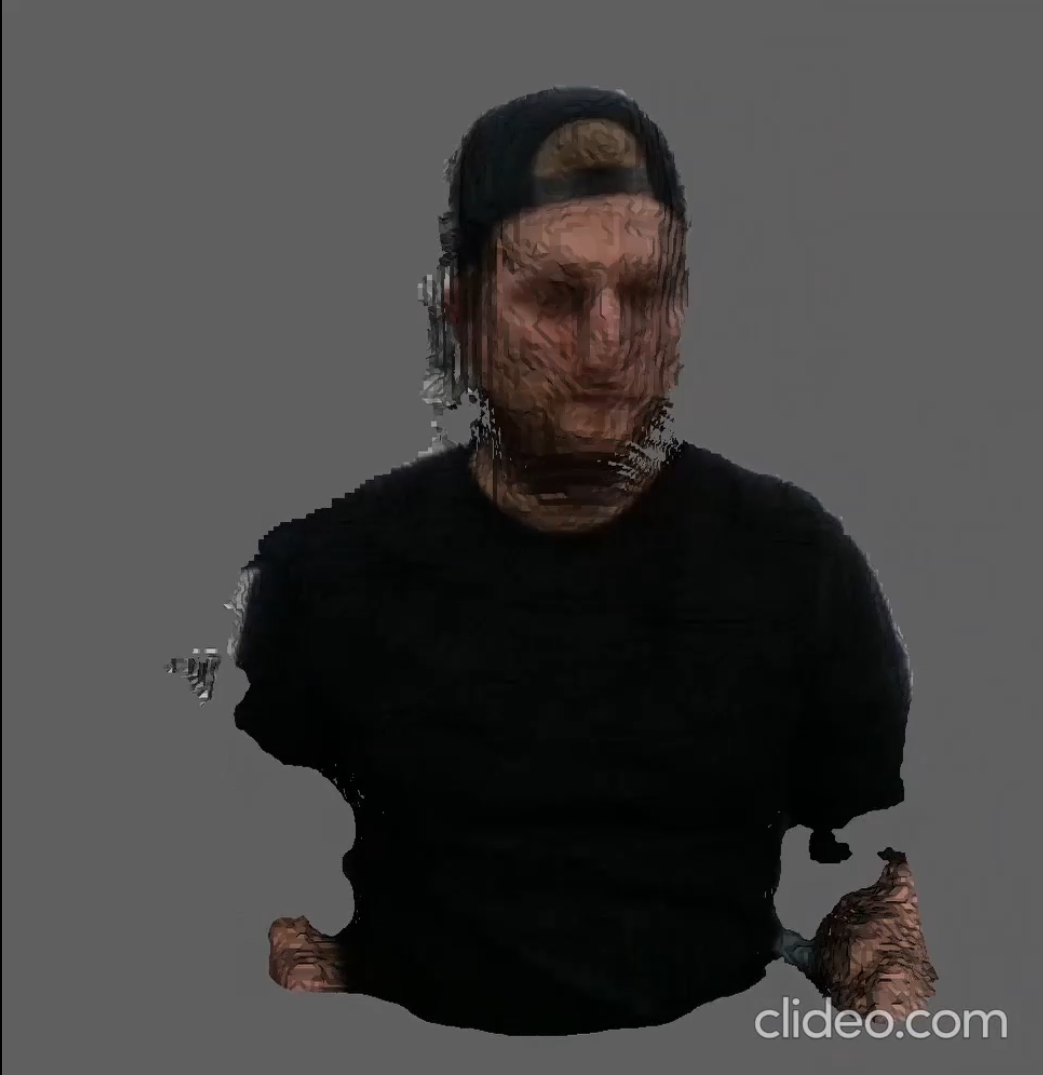
\includegraphics[width=0.65\linewidth]{imgs/res1}
\end{center}
 \caption{Result with using only one camera}
 \label{fig:res1}
\end{figure}

\begin{figure}[t]
\begin{center}
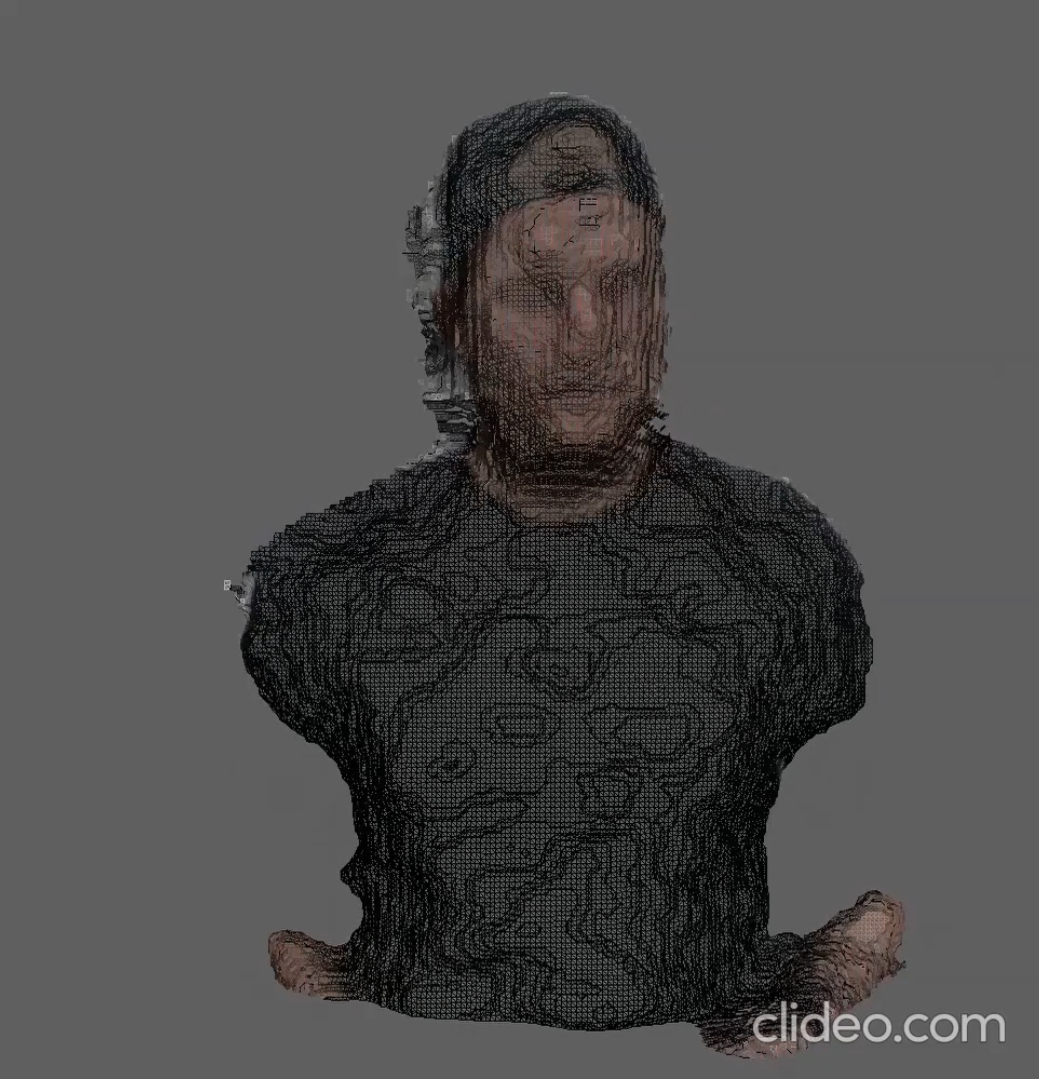
\includegraphics[width=0.65\linewidth]{imgs/res2}
\end{center}
 \caption{Triangulation result with using only one camera}
 \label{fig:res2}
\end{figure}

\begin{figure}[t]
\begin{center}
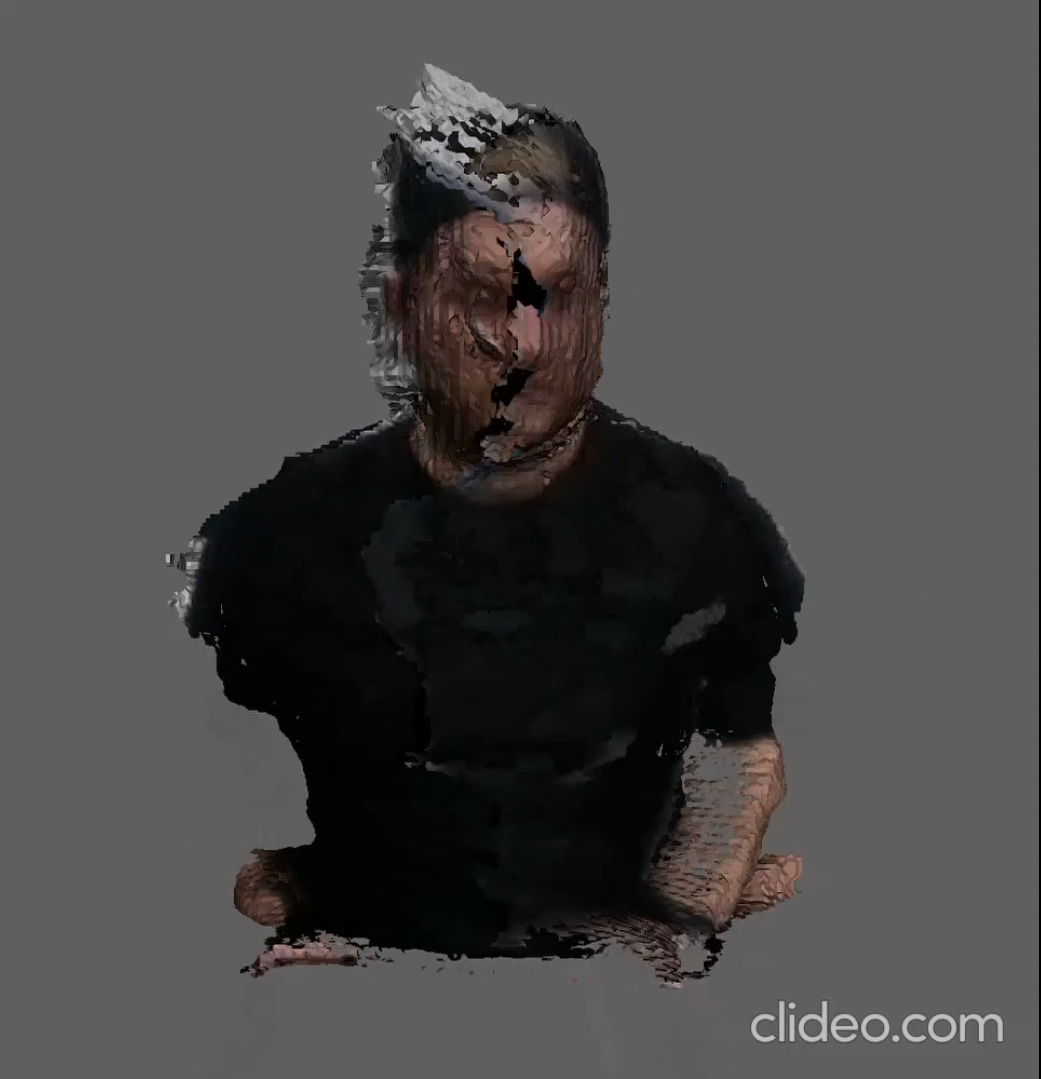
\includegraphics[width=0.65\linewidth]{imgs/res3}
\end{center}
 \caption{Result with using three cameras}
 \label{fig:res3}
\end{figure}

\begin{table}[h!]
  \begin{center}
    \begin{tabular}{c|c|c|c p{4cm}}
      \textbf{Algorithm} & \textbf{Iterations} & \textbf{Duration [ms]} & \textbf{MSE}\\
      \hline
      Procrustes (A)  & 1 & 8 - 20 & \textless 0.7 - 1.73\\
      Point-to-Point (A) & 1 - 20 & 900 - 1000 & \textless 0.1\\
      Procrustes (C) & 1 & 20 - 40 & 0.25 - 1.29\\
      Point-to-Point (C) & 1 - 20 & 18000 - 22000 & \textless 0.1\\
    \end{tabular}
     \caption{Comparisons between different optimization algorithms in terms of iterations, duration and MSE (Mean Squared Error). A = ArUco, C = ChArUco}
     \label{tab:camera-calibration}
  \end{center}
\end{table}

\begin{table}[h!]
  \begin{center}
    \begin{tabular}{c|c|c|c p{4cm}}
      \textbf{Algorithm} & \textbf{Resolution [mm]} & \textbf{Voxels} & \textbf{Duration [ms]}\\
      \hline
      Voxelgrid & 20 & 125,000 & \textless 1\\
      Voxelgrid & 10 & 1,000,000 & \textless 1\\
      Voxelgrid & 5 & 8,000,000 & 5\\
      Voxelgrid & 4 & 15,625,000 & 20\\
      Voxelgrid & 3 & 37,000,000 & 50\\
    \end{tabular}
     \caption{Time comparisons for calculating voxelgrid of different voxel resolutions as well as the number of voxels used. The voxelgrid measured 1 meter x 1 meter x 1 meter.}
     \label{tab:voxelgrid}
  \end{center}
\end{table}

\begin{table}[h!]
  \begin{center}
    \begin{tabular}{c|c|c p{4cm}}
      \textbf{Resolution [mm]} & \textbf{Duration [ms]} & \textbf{Voxels}\\
      \hline
      20 & \textless 1 & 7,000 - 10,000\\
      10 & \textless 1 & 40,000 - 45,000\\
      5 & 15 & 200,000 - 250,000\\
      4 & 35 & 380,000 - 420,000\\
      3 & 80 & 600,000 - 800,000\\
    \end{tabular}
     \caption{Time comparisons for running the Marching Cubes on different voxel resolutions. The number of triangles generated are also displayed.}
     \label{tab:table3}
  \end{center}
\end{table}

%------------------------------------------------------------------------
\section{Future Work and Conclusion}
Since we optimized for pose parameters for a limited number of markers, one of the further improvements that we can do in camera calibration is to use more correspondences which can found for example by using Nearest Neighbor Search and then use the Global Alignment techniques like Iterative Closest Points (ICP).

%------------------------------------------------------------------------
\section{Group Member Contributions}

\newpage
{\small
\bibliographystyle{ieee_fullname}
\bibliography{egbib}
}

\end{document}
